\documentclass[12pt]{article}

\usepackage{amsmath}
\usepackage{amssymb}
\usepackage{physics}
\usepackage{enumitem}
\usepackage{tikz}
\usetikzlibrary{arrows.meta,calc,angles,quotes,decorations.pathmorphing}
\usepackage{geometry}
\geometry{margin=1in}

\begin{document}

\begin{center}
{\Large \textbf{SET 17 — Ultra Advanced (Fully Stabilized Length-Preserved Version)}}
\end{center}

\begin{enumerate}[leftmargin=*]

%========================================================
\item A small bead of mass $m$ can slide without friction on a circular ring of radius $R$.  
The ring is fixed in a vertical plane and rotates with constant angular speed $\omega$ about its vertical diameter.  

Gravitational acceleration $g$ acts vertically downward.  
In the rotating frame of the ring, pseudo forces must be considered along with gravity.  

Determine the critical angular speed at which the lowest equilibrium position loses stability and two new symmetric equilibrium positions appear on either side of the vertical diameter.

\begin{center}
\begin{tikzpicture}[scale=1]
\draw (0,0) circle(2);
\draw[dashed] (0,2)--(0,-2);
\fill (0,-2) circle(2pt);
\draw[->] (0,2.5)--(0,3.2) node[right]{$\omega$};
\end{tikzpicture}
\end{center}

\begin{enumerate}
\item $\sqrt{\dfrac{g}{R}}$
\item $\sqrt{\dfrac{2g}{R}}$
\item $\sqrt{\dfrac{g}{2R}}$
\item $\sqrt{\dfrac{3g}{R}}$
\end{enumerate}

%========================================================
\item A solid sphere of mass $M$ and radius $r$ rolls without slipping down a wedge of mass $m$.  
The wedge rests on a perfectly smooth horizontal surface and is free to move.  

The inclination of the wedge with horizontal is $\theta$.  
Assume pure rolling constraint between sphere and wedge and no slipping at the contact surface.  

Taking into account translational motion of the wedge, rolling constraint, and conservation of horizontal momentum, determine the acceleration of the centre of mass of the sphere relative to the ground.

\begin{center}
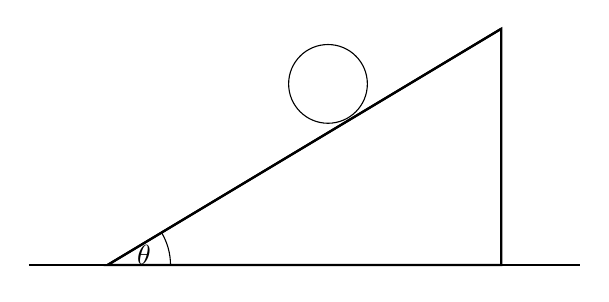
\begin{tikzpicture}[scale=1]
\draw[thick] (0,0)--(7,0);
\coordinate (A) at (1,0);
\coordinate (B) at (6,0);
\coordinate (C) at (6,3);
\draw[thick] (A)--(B)--(C)--cycle;
\draw[thick] (A)--(C);
\draw (3.8,2.3) circle(0.5);
\draw pic["$\theta$", draw=black, angle radius=0.8cm]
{angle = B--A--C};
\end{tikzpicture}
\end{center}

\begin{enumerate}
\item $\displaystyle \frac{g\sin\theta}{\frac{7}{5}+\frac{M}{m}}$
\item $\displaystyle \frac{g\sin\theta}{\frac{7}{5}}$
\item $\displaystyle \frac{g\sin\theta}{2+\frac{M}{m}}$
\item $\displaystyle \frac{g\sin\theta}{\frac{5}{7}+\frac{M}{m}}$
\end{enumerate}

%========================================================
\item A particle of mass $m$ moves under the influence of a central force
\[
F(r)=-\frac{k}{r^2}+\frac{3\alpha}{r^4}
\]
where $k>0$ and $\alpha>0$.  

The motion is nearly circular about radius $r_0$.  
Using effective potential method and small radial oscillation approximation, determine the ratio of radial oscillation frequency $\omega_r$ to angular frequency $\omega_\theta$.

\begin{enumerate}
\item $\sqrt{1-\dfrac{3\alpha}{k r_0^2}}$
\item $\sqrt{1-\dfrac{6\alpha}{k r_0^2}}$
\item $\sqrt{1+\dfrac{3\alpha}{k r_0^2}}$
\item $\sqrt{1-\dfrac{\alpha}{k r_0^2}}$
\end{enumerate}

%========================================================
\item A point charge $q$ is placed at a distance $a$ from the centre $O$ of a grounded conducting sphere of radius $R$ where $a>R$.  

Using method of images and electrostatic boundary conditions, determine the magnitude of electrostatic force acting on the charge $q$.

\begin{center}
\begin{tikzpicture}[scale=1]
\draw (0,0) circle(2);
\fill (0,0) circle(2pt);
\node[below left] at (0,0) {$O$};
\draw[dashed] (0,0)--(2,0);
\node[below] at (1,0) {$R$};
\coordinate (Q) at (4.5,0);
\fill (Q) circle(2pt);
\node[right] at (Q) {$q$};
\draw[dashed] (0,0)--(Q);
\node[below] at (2.3,0) {$a$};
\end{tikzpicture}
\end{center}

\begin{enumerate}
\item $\dfrac{1}{4\pi\epsilon_0}\dfrac{q^2 R a}{(a^2-R^2)^2}$
\item $\dfrac{1}{4\pi\epsilon_0}\dfrac{q^2 R}{(a^2-R^2)}$
\item $\dfrac{1}{4\pi\epsilon_0}\dfrac{q^2 R^2}{a^2(a^2-R^2)}$
\item $\dfrac{1}{4\pi\epsilon_0}\dfrac{q^2}{(a-R)^2}$
\end{enumerate}

%========================================================
\item A photon of energy $3mc^2$ is incident on a free electron initially at rest.  

Using full relativistic Compton scattering formalism and conservation of four-momentum, determine the maximum kinetic energy gained by the electron.

\begin{enumerate}
\item $\dfrac{18}{7}mc^2$
\item $\dfrac{9}{10}mc^2$
\item $\dfrac{3}{4}mc^2$
\item $\dfrac{2}{3}mc^2$
\end{enumerate}

%========================================================
\item A satellite of mass $m$ is in circular orbit of radius $R$ around Earth.  

Its orbital speed is suddenly reduced to $\frac{1}{\sqrt{2}}$ times the original circular speed without changing its instantaneous direction of motion.  

Neglect atmospheric drag and perturbations.  
Determine the nature of the new orbit formed after velocity reduction.

\begin{enumerate}
\item Elliptical with apogee $R$
\item Elliptical with perigee $R$
\item Circular of radius $\frac{R}{2}$
\item Escape trajectory
\end{enumerate}

%========================================================
\item A glass slab of refractive index $n$ moves with uniform velocity $u \ll c$ parallel to its surface.  

A light ray is incident normally on the slab in the laboratory frame.  

Using relativistic velocity transformation to first order in $u/c$, determine the angle of emergence in laboratory frame.

\begin{center}
\begin{tikzpicture}
\draw[thick] (0,0)--(6,0)--(6,2)--(0,2)--cycle;
\draw[->] (3,3)--(3,2);
\draw[->] (0,-0.5)--(1.5,-0.5) node[right]{$u$};
\end{tikzpicture}
\end{center}

\begin{enumerate}
\item $0$
\item $\dfrac{u}{c}\left(1-\dfrac{1}{n}\right)$
\item $\dfrac{u}{c}(n-1)$
\item $\dfrac{nu}{c}$
\end{enumerate}

%========================================================
\item A particle of mass $m$ moves in one dimensional potential
\[
U(x)=ax^4-bx^2
\]
where $a>0$ and $b>0$.  

The particle performs small oscillations about one of the stable equilibrium positions.  
Determine the angular frequency of small oscillations by proper Taylor expansion about equilibrium.

\begin{enumerate}
\item $\sqrt{\dfrac{2b}{m}}$
\item $\sqrt{\dfrac{4b}{m}}$
\item $\sqrt{\dfrac{8b}{m}}$
\item $\sqrt{\dfrac{b}{m}}$
\end{enumerate}

%========================================================
\item Two long parallel conducting rails are connected at one end forming a closed circuit.  

A conducting rod of mass $m$, length $l$, and resistance $R$ can slide without friction on the rails.  

A uniform magnetic field $B$ exists perpendicular to the plane of rails (out of page).  

The rod is given initial speed $v_0$ away from the fixed end.  

Determine the total distance travelled by the rod before coming to rest due to magnetic braking.

\begin{enumerate}
\item $\dfrac{mRv_0}{B^2l^2}$
\item $\dfrac{mv_0}{B^2l^2R}$
\item $\dfrac{mRv_0}{2B^2l^2}$
\item $\dfrac{mv_0^2R}{B^2l^2}$
\end{enumerate}

%========================================================
\item A uniform rod of length $L$ and mass $m$ is pivoted at one end.  

A projectile of mass $\frac{m}{2}$ moving horizontally with speed $v$ strikes the lower end of the rod and gets embedded.  

Using angular momentum conservation about pivot and energy considerations for full vertical circle, determine the minimum value of $v$ such that the system just completes a full revolution.

\begin{enumerate}
\item $\sqrt{\dfrac{27gL}{4}}$
\item $\sqrt{\dfrac{9gL}{2}}$
\item $\sqrt{6gL}$
\item $\sqrt{\dfrac{15gL}{2}}$
\end{enumerate}

%========================================================
\item A long solenoid of radius $R$ carries time varying current
\[
I=I_0\sin\omega t.
\]

A circular conducting loop of radius $r<R$ is placed coaxially inside the solenoid.  

Determine the amplitude of induced electric field at distance $r$ from the axis.

\begin{enumerate}
\item $\dfrac{\mu_0 n \omega I_0 r}{2}$
\item $\dfrac{\mu_0 n \omega I_0 R}{2}$
\item $\dfrac{\mu_0 n I_0 r}{2}$
\item $\dfrac{\mu_0 n \omega I_0 r^2}{2}$
\end{enumerate}

%========================================================
\item A block of mass $m$ is attached between two identical springs of spring constant $k$ each, fixed to rigid walls.  

The block oscillates on a frictionless surface.  
Now the entire system is accelerated horizontally with constant acceleration $a$.  

Determine the new equilibrium displacement of the block from the original central position.

\begin{enumerate}
\item $\dfrac{ma}{2k}$
\item $\dfrac{ma}{k}$
\item $\dfrac{2ma}{k}$
\item Zero
\end{enumerate}

%========================================================
\item A hydrogen atom initially in ground state absorbs a photon and transitions to $n=3$.  

Using Bohr model energy levels, determine the ratio of wavelength of absorbed photon to the wavelength of the first Balmer line.

\begin{enumerate}
\item $\dfrac{27}{20}$
\item $\dfrac{4}{5}$
\item $\dfrac{5}{4}$
\item $\dfrac{9}{8}$
\end{enumerate}

%========================================================
\item A parallel plate capacitor of plate area $A$ and separation $d$ is connected to a battery of voltage $V$.  

A dielectric slab of dielectric constant $k$ is slowly inserted so that it occupies exactly half the volume between the plates while battery remains connected.  

Determine the net work done by the external agent during the insertion.

\begin{enumerate}
\item $\dfrac{1}{4}CV^2(k-1)$
\item $\dfrac{1}{2}CV^2(k-1)$
\item $\dfrac{1}{8}CV^2(k-1)$
\item $\dfrac{1}{4}CV^2\left(1-\dfrac{1}{k}\right)$
\end{enumerate}

%========================================================
\item Two identical coherent sources separated by distance $d$ emit light of wavelength $\lambda$.  

On a distant screen at distance $D$, the central maximum intensity is $I_0$.  

If the intensity of one source is reduced to one-fourth while coherence is maintained, determine the new central intensity.

\begin{enumerate}
\item $\dfrac{9}{16}I_0$
\item $\dfrac{25}{16}I_0$
\item $\dfrac{5}{4}I_0$
\item $\dfrac{4}{9}I_0$
\end{enumerate}

\end{enumerate}

\end{document}